\documentclass{standalone}

\usepackage{tikz}
\usetikzlibrary{
    decorations.markings,
    decorations.pathmorphing,
    decorations.text,
}


\begin{document}
\noindent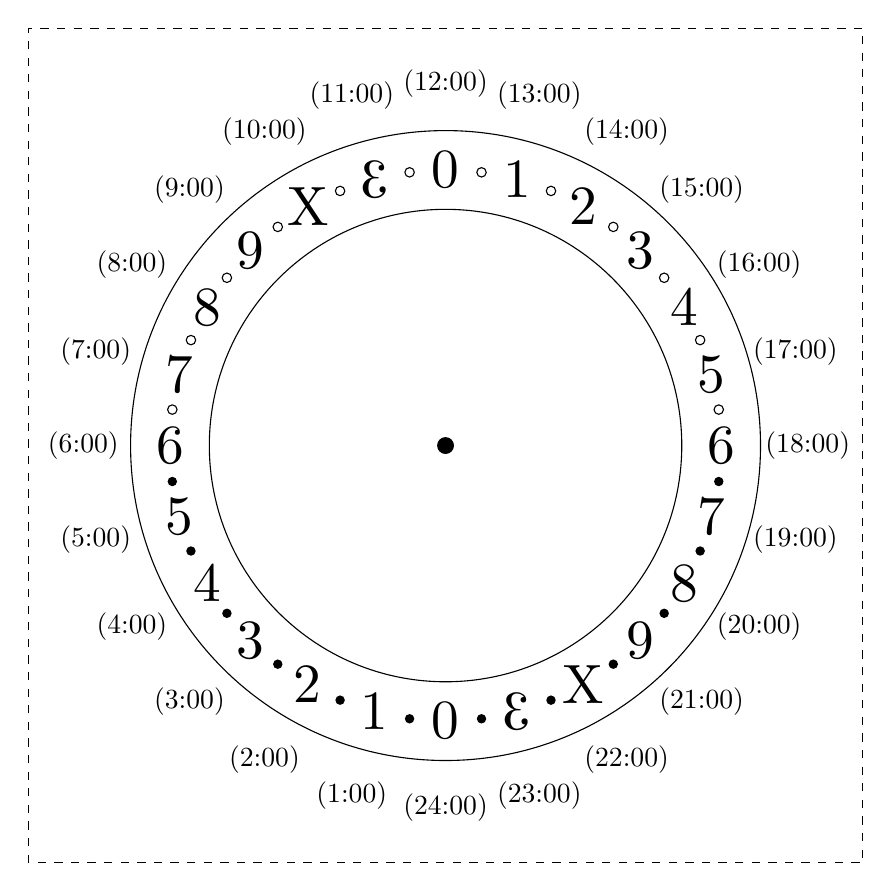
\begin{tikzpicture}
    % Border
    \draw[dashed] (-53mm,-53mm) rectangle (53mm,53mm);
    % Middle
    \draw[fill] (0,0) circle [radius=1mm];
    % Numerals
    \foreach \angle/\label/\xscale in {%
            270/0/1,255/1/1,240/2/1,225/3/1,210/4/1,195/5/1,%
            180/6/1,165/7/1,150/8/1,135/9/1,120/X/1,105/3/-1%
    } {
        \node[scale=2,inner sep=0pt,xscale=\xscale]
            at (\angle:35mm) {\label};
        \node[scale=2,inner sep=0pt,xscale=\xscale]
            at (\angle-180:35mm) {\label};
    }
    % Dots
    \foreach \angle in {0,15,...,165} {
        \draw (\angle+7.5:35mm)     circle (0.6mm);
        \fill (\angle+7.5+180:35mm) circle (0.6mm);
    }

    % Rim borders
    \draw (0,0) circle [radius=40mm];
    \draw (0,0) circle [radius=30mm];
    % Labels
    \foreach[count=\label] \angle in {255,240,...,-90} {
        \node at (\angle:46mm) {(\label:00)};
    }

\end{tikzpicture}

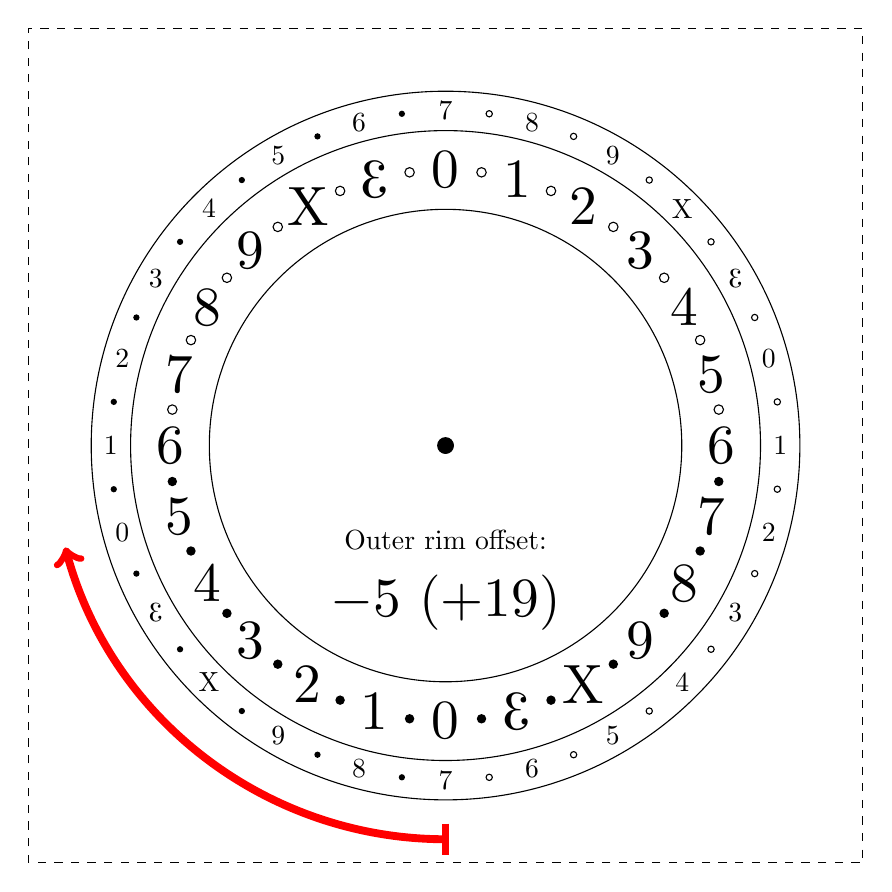
\begin{tikzpicture}
    % Border
    \draw[dashed] (-53mm,-53mm) rectangle (53mm,53mm);
    % Middle
    \draw[fill] (0,0) circle [radius=1mm];

    % INNER RIM
    % Numerals
    \foreach \angle/\label/\xscale in {%
            270/0/1,255/1/1,240/2/1,225/3/1,210/4/1,195/5/1,%
            180/6/1,165/7/1,150/8/1,135/9/1,120/X/1,105/3/-1%
    } {
        \node[scale=2,inner sep=0pt,xscale=\xscale]
            at (\angle:35mm) {\label};
        \node[scale=2,inner sep=0pt,xscale=\xscale]
            at (\angle-180:35mm) {\label};
    }
    % Dots
    \foreach \angle in {0,15,...,165} {
        \draw (\angle+7.5:35mm)     circle (0.6mm);
        \fill (\angle+7.5+180:35mm) circle (0.6mm);
    }
    
    % OUTER RIM
    % Numerals
    \foreach \angle/\label/\xscale in {%
            270/0/1,255/1/1,240/2/1,225/3/1,210/4/1,195/5/1,%
            180/6/1,165/7/1,150/8/1,135/9/1,120/X/1,105/3/-1%
    } {
        \node[scale=1,inner sep=0pt,xscale=\xscale]
            at (\angle-75:42.5mm) {\label};
        \node[scale=1,inner sep=0pt,xscale=\xscale]
            at (\angle-75-180:42.5mm) {\label};
    }
    % Dots
    \foreach \angle in {0,15,...,165} {
        \draw (\angle-75-7.5:42.5mm)     circle (0.4mm);
        \fill (\angle-75-7.5+180:42.5mm) circle (0.4mm);
    }

    % Rim borders
    \draw (0,0) circle [radius=45mm];
    \draw (0,0) circle [radius=40mm];
    \draw (0,0) circle [radius=30mm];

    % Rotation
    \draw[red,line width=1mm]    (270:48mm) -- (270:52mm);
    \draw[red,line width=1mm,->] (270:50mm) arc (270:270-75:50mm);

    % Label
    \node at (270:12mm) {Outer rim offset:};
    \node[scale=2] at (270:20mm) {$-5$ ($+19$)};
\end{tikzpicture}
\end{document}
